\begin{defi}[Polynômes de \textsc{Legendre}]
    On appelle famille des \emph{polynômes de \nom{Legendre}} la suite de polynômes $\suite{\Leg}{n}{n \in \Ne}$ définie par
    $$\Leg_n(X) \defeq \frac{1}{2^n} \sum_{k=0}^{n} \binom{n}{k}^2 (X-1)^{n-k}(X+1)^{k}.$$
\end{defi}

\marginnote[0cm]{
    Voir aussi...
}

\begin{exercice}
    \source{\cite{exos_oraux} p. 25} 
    \begin{questions}
        \item Montrer que $\Leg_n(X) = \frac{1}{2^n \fact{n}} \left[ \big(X^2-1\big)^n \right]^{(n)}$. En déduire la parité de $\Leg_n$ et l'égalité $\sum\limits_{k=0}^n \binom{n}{k}^2 = \binom{2n}{n}$.
        \item Soit $n \in \Ne$, montrer que $\Leg_n(X)$ est scindé à racines simples dans $\interoo{-1}{1}$. 
        \item Montrer que pour tout $n \in \N$, $$\big(X^2-1\big) \Leg''_n(X) + 2X \Leg'_n(X) = n(n+1) \Leg_n.$$
    \end{questions}
\end{exercice}  

\begin{elemsolution}
    Pour montrer que $\Leg_n(X)$ est scindé à racines simples dans $\interoo{-1}{1}$, raisonner par récurrence et penser à \textsc{Rolle}. 
\end{elemsolution}

\begin{marginfigure}[-11.5cm]
    \centering
	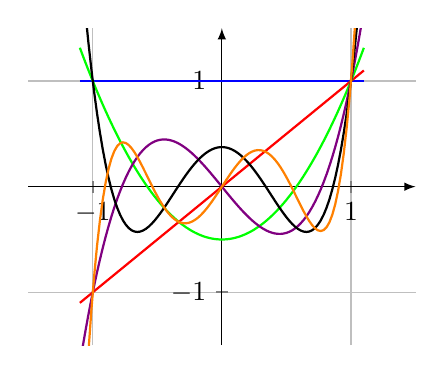
\begin{tikzpicture}
    \begin{axis}[width=6.5cm,
        axis lines=middle,
        inner axis line style={-latex},
        grid=major,
        xmin=-1.5, xmax=1.5,
        ymin=-1.5, ymax=1.5,
        % xlabel=$x$, xlabel style={right},
        % ylabel=$y$, ylabel style={above},
        tick style={thick},
        ticklabel style={font=\normalsize},
        xtick={-1, 0, 1}, 
        ytick={-1, 0, 1},
        % legend entries={0.5x},
            legend style={
            at={(1.05,0.4)},
            anchor=north,
            legend columns=1},
            legend cell align={left}
    ]
    
    \def\a{-1.1}
    \def\b{1.1}
    
    \addplot[blue,thick,samples=100,domain=\a:\b] {1};
    \addplot[red,thick,samples=100,domain=\a:\b] {x};
    \addplot[green,thick,samples=100,domain=\a:\b] {1/2*(3*x^2-1)};
    \addplot[violet,thick,samples=100,domain=\a:\b] {1/2*(5*x^3-3*x)};
    \addplot[black,thick,samples=100,domain=\a:\b] {1/8*(35*x^4-30*x^2+3)};
    \addplot[orange,thick,samples=100,domain=\a:\b] {1/8*(63*x^5-70*x^3+15*x)};
    
   % \legend{$\Leg_0$, 
   %         $\Leg_1$,
%            $\Leg_2$,
%            $\Leg_3$,
 %           $\Leg_4$,
  %          $\Leg_5$
   %         }
    \end{axis}
\end{tikzpicture}
	\caption*{\centering Les premiers polynômes de \textsc{Legendre}}
	\small
	\begin{align*}
	    \color{blue} \Leg_0 = 1 \\
	    \color{red} \Leg_1 = x \\
	    \color{green} \Leg_2 = \frac{1}{2}\big(3x^2-1\big) \\
	    \color{purple} \Leg_3 = \frac{1}{2}\big(5x^3-3x\big) \\
	    \color{black} \Leg_4 = \frac{1}{8}\big(35x^4-30x^2+3\big) \\
	    \color{orange} \Leg_5 = \frac{1}{8}\big(63x^5-70x^3+15x\big)
	\end{align*}
\end{marginfigure}

